\subsection{HTTP header size}
\label{subsec:header_size}

HTTP/2 uses HPACK \cite{hpack} as a header compression mechanism in order to decrease the amount of data for repetitive HTTP header information. Figure \ref{fig:headersize} shows the difference between HTTP/2 and HTTP/1.1 regarding the amount of header depending on the amount of clients.

\begin{figure}[H]
	\centering
	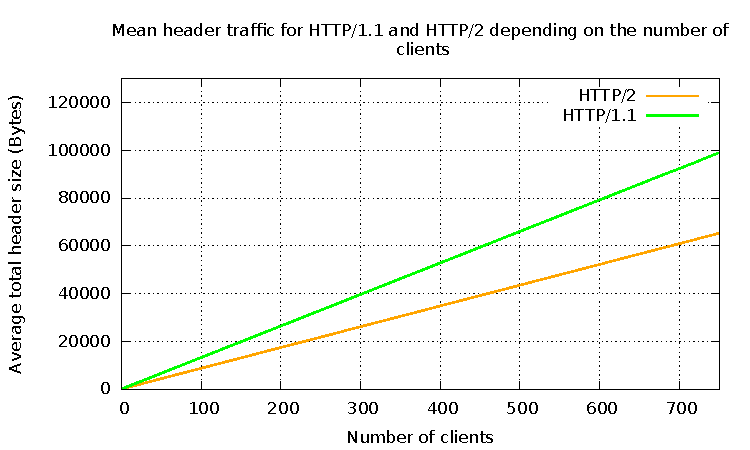
\includegraphics[scale=1,trim=0.0cm .0cm .0cm .0cm,clip]{images/headertraffic.pdf}
	\caption{header traffic in bytes for HTTP1.1 and HTTP/2}
	\label{fig:headersize}
\end{figure}

The result is a linear graph for both versions with a higher rate of growth for HTTP/1.1. It turns out that in our measurement set-up the amount of traffic produced to transmit HTTP headers is approximately 30\% lower for HTTP/2 compared to HTTP/1.1. 
